
%
%	Section 2
%

\section{Super-Kamiokande}\label{Section_002}
\Headerfooter{Super-Kamiokande}

\subsection{Super-Kamiokande}
\vs\hs The Super-Kamiokande (SK)~\cite{2003Fukuda} is the experiment held in Kamioka, Gifu, Japan, with the large water Cherenkov detector placed in 1,000 m underground, 2,700 m water equivalent overburden.
The overview of the SK detector is shown in Figure~\ref{002_F01_SK}.
The SK stands for ``Super-Kamioka Neutrino Detection Experiment'' and ``Super-Kamioka Nucleon Decay Experiment''.
The rate of cosmic ray muon is reduced by a factor of 10$^{\text{5}}$ compared to that of the ground level.\\

\begin{figure}[h]
	\centering
	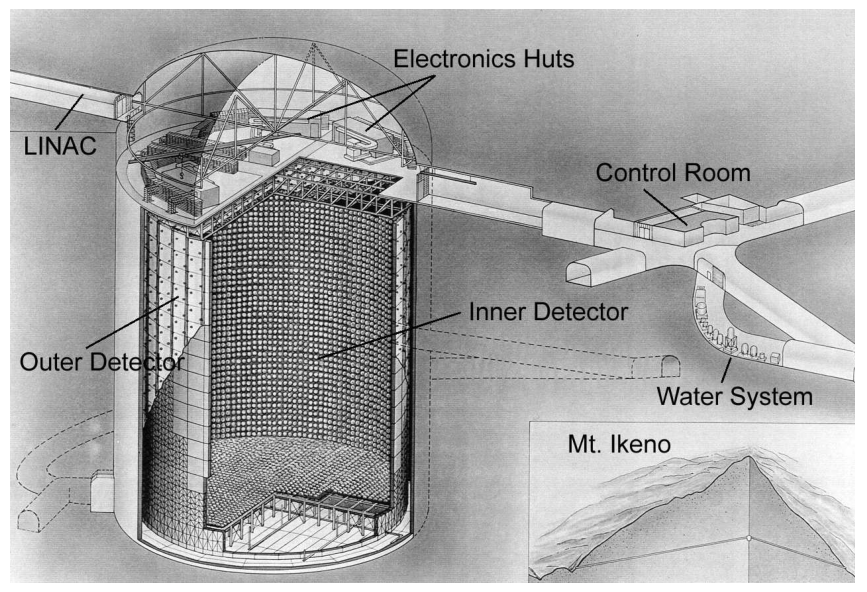
\includegraphics[width=15cm]{Figures/002/F01_SK}
	\caption[Overview of the Super-Kamiokande detector]{\label{002_F01_SK} Overview of the SK detector~\cite{2003Fukuda}.}
\end{figure}

\hs The SK detector consists of the stainless-steel cylindrical tank with a diameter of 39.3 m and a height of 41.4 m and 50 kilotons ultrapure water.
The tank is separated into the inner detector (ID) and the outer detector (OD) by stainless-steel frames (supermodule frames).
The cross section of the SK detector and the overview of supermodule frames are shown in Figure~\ref{002_F02_SK_SM}.
The diameter of ID, the height of ID and the volume of ID (the fiducial volume) is 33.8 m, 36.2 m and 32 kilotons (22.5 kilotons), respectively.
In ID, 11,129 20-inch (50 cm) photomultiplier tubes (PMTs) are installed.
The gaps between ID PMTs are covered by black polyethylene terephthalate sheets.
The sheets separate ID and OD optically and suppress the reflection at the surface of the ID wall.
Moreover, the sheets reduce low energy events by radioactive backgrounds occurring behind the PMTs.
On the other hand, in OD, 1,885 8-inch (20 cm) PMTs are installed.
OD volume is covered by white Tyvek sheets manufactured by DuPont.
The Tyvek sheets have high reflectivity and enhance the light collection efficiency in OD.

\begin{figure}[tbp]
	\centering
	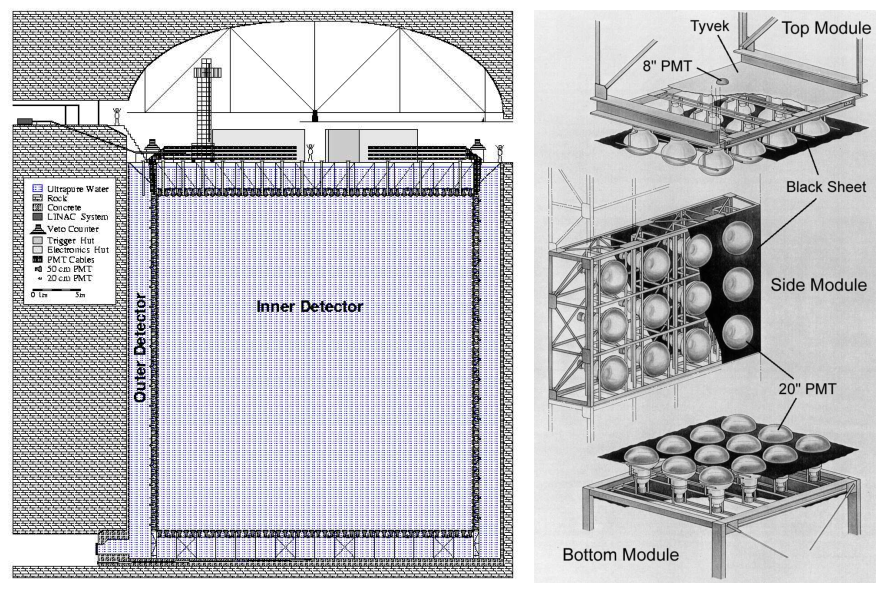
\includegraphics[width=15cm]{Figures/002/F02_SK_SM}
	\caption[Cross section of the SK detector and overview of supermodule frames]{\label{002_F02_SK_SM} Cross section of the SK detector (left) and overview of supermodule frames (right)~\cite{2003Fukuda}.}
\end{figure}

\subsection{ID PMT}
\vs\hs The schematic view of the ID PMT is shown in Figure~\ref{002_F03_IDPMT}.
The number of ID PMTs is 7,650 on the barrel (side walls), 1,740 on the top and 1,739 on the bottom, thus the effective photocathode coverage of ID is 40\%.
The role of ID PMTs is to reconstruct the energy, generated position, direction and the kind of the charged particles.
Figure~\ref{002_F04_IDPMTQE} shows the quantum efficiency of the ID PMT photocathode as a function of wavelength.
The material of photocathode is bialkali (Sb-K-Cs) and the quantum efficiency is about 21\% at 360 - 400 nm.
Figure~\ref{002_F05_IDPMT1pe} shows the single photoelectron pulse height distribution of the ID PMT.
The peak around zero ADC count is caused by PMT dark current.
Figure~\ref{002_F06_IDPMTt} shows the relative transit time distribution for a typical ID PMT tested using 410 nm wavelength light at the single photoelectron intensity level.
The 1$\sigma$ of transit time for a single photoelectron signal is 2.16 ns.

\begin{figure}[tbp]
	\centering
	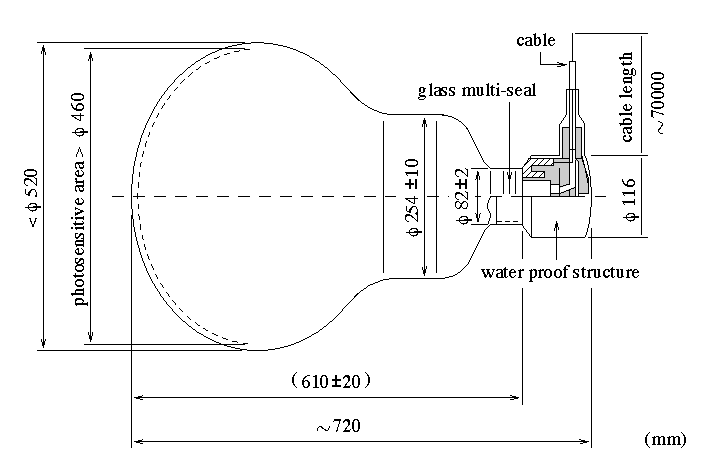
\includegraphics[width=12cm]{Figures/002/F03_IDPMT}
	\caption[Schematic view of the ID PMT]{\label{002_F03_IDPMT} Schematic view of the ID PMT~\cite{2003Fukuda}.}
\end{figure}

\begin{figure}[tbp]
	\centering
	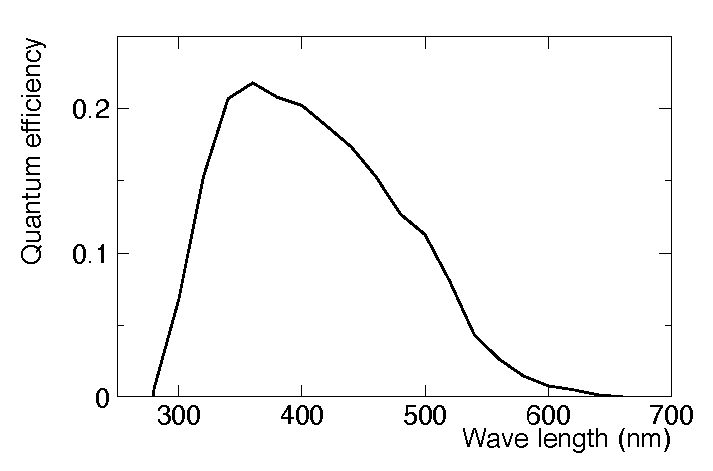
\includegraphics[width=12cm]{Figures/002/F04_IDPMTQE}
	\caption[Quantum efficiency of the ID PMT photocathode as a function of wavelength]{\label{002_F04_IDPMTQE} Quantum efficiency of the ID PMT photocathode as a function of wavelength~\cite{2003Fukuda}. The material of ID PMT photocathode is bialkali (Sb-K-Cs).}
\end{figure}

\begin{figure}[tbp]
	\centering
	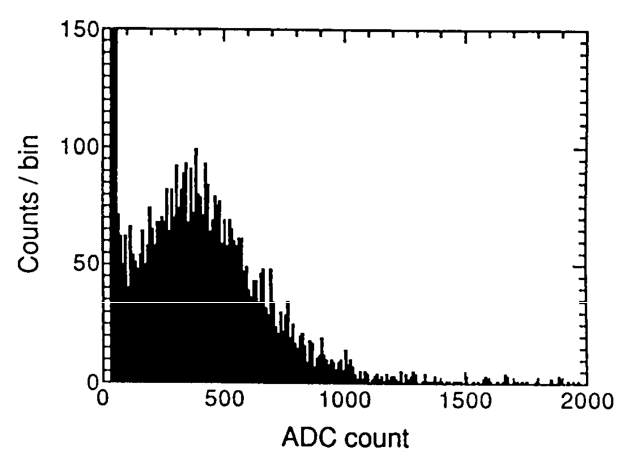
\includegraphics[width=12cm]{Figures/002/F05_IDPMT1pe}
	\caption[Single photoelectron pulse height distribution of the ID PMT]{\label{002_F05_IDPMT1pe} Single photoelectron pulse height distribution of the ID PMT~\cite{2003Fukuda}. The peak around zero ADC count is caused by PMT dark current.}
\end{figure}

\begin{figure}[tbp]
	\centering
	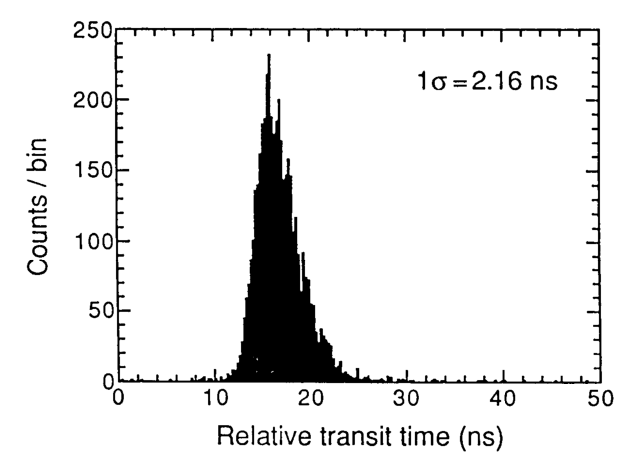
\includegraphics[width=12cm]{Figures/002/F06_IDPMTt}
	\caption[Relative transit time distribution for a typical ID PMT tested using 410 nm wavelength light at the single photoelectron intensity level]{\label{002_F06_IDPMTt} Relative transit time distribution for a typical ID PMT tested using 410 nm wavelength light at the single photoelectron intensity level~\cite{2003Fukuda}.}
\end{figure}

\subsection{OD PMT}
\vs\hs The number of OD PMTs is 1,275 on the barrel, 302 on the top and 308 on the bottom.
To compensate the small number of OD PMTs, wavelength shifting (WS) plate is attached to each OD PMT.
The WS plate is square acrylic panel with a side of 60 cm and a thickness of 1.3 cm, doped with 50 mg$/$L of bis-MSB (C$_{\text{24}}$H$_{\text{22}}$).
The WS plate absorbs UV light, and then emit photons in the blue - green.
OD PMT with bialkali photocathode is more sensitive to blue - green photons than UV photons.
Therefore, the light collection efficiency is improved by about a factor of 1.5 compared to without WS plates.
The timing resolution of OD PMTs with WS plates is 15 ns (FWHM), which is poorer than that of ID PMTs.
However, OD was optimized as a veto counter and the poorer timing resolution is less important.
Figure~\ref{002_F07_IDODPMT} shows the positional relationship of ID PMTs and OD PMTs in a supermodule frame.
Basically, in a supermodule frame, 12 ID PMTs and 2 OD PMTs are attached.

\begin{figure}[h]
	\centering
	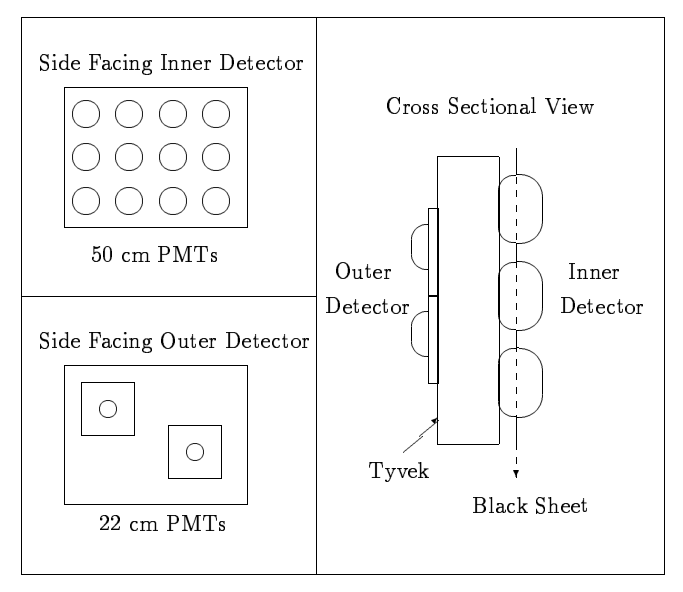
\includegraphics[width=10cm]{Figures/002/F07_IDODPMT}
	\caption[Positional relationship of ID PMTs and OD PMTs in a supermodule frame]{\label{002_F07_IDODPMT} Positional relationship of ID PMTs and OD PMTs in a supermodule frame~\cite{1997ZoaPhD}. 12 ID PMTs and 2 OD PMTs are attached in a supermodule frame, basically.}
\end{figure}

\subsection{Helmholtz coils}
\vs\hs The geomagnetic field would affect photoelectron trajectories and timing in the PMTs.
Therefore, 26 sets of horizontal and vertical Helmholtz coils are deployed around the inner surface of the tank to reduce the geomagnetic field.
Figure~\ref{002_F08_Coil} shows the schematic view of Helmholtz coils.
The average geomagnetic field intensity without Helmholtz coils is about 450 mG~\cite{2003Fukuda}.
The average field intensity can be reduced to 32 mG with Helmholtz coils, resulting that the deviation in the collection efficiency of photoelectrons is 2\%~\cite{2014AbeCalib}.

\begin{figure}[tbp]
	\centering
	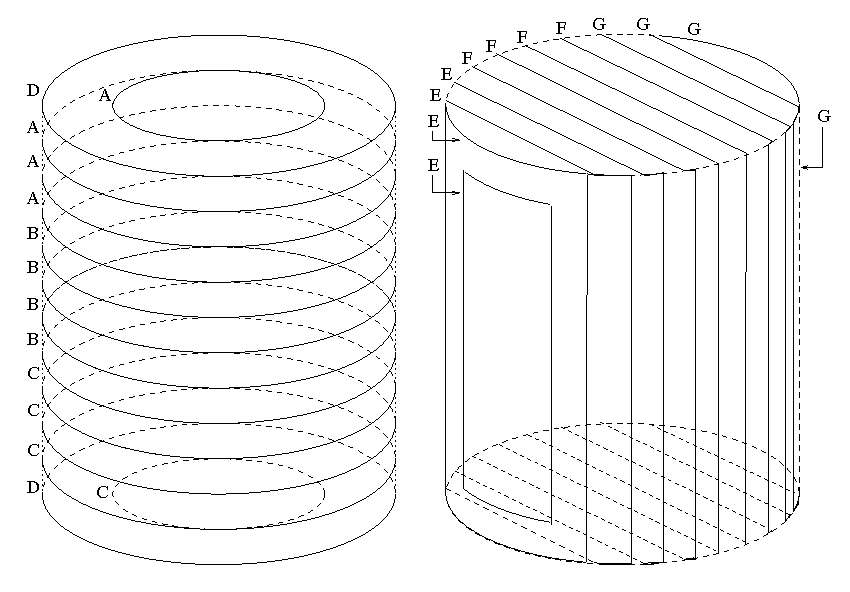
\includegraphics[width=12cm]{Figures/002/F08_Coil}
	\caption[Schematic view of Helmholtz coils]{\label{002_F08_Coil} Schematic view of Helmholtz coils~\cite{1998YamaguchiPhD}.}
\end{figure}

\newpage
